\chapter{The Parton Shower}

Parton showers are approximations of what is seen in the detectors (stable particles) to the hard scattering. The word "hard", means the process involves a transfer of large momentum, in which the parons are splitting and branching.  
% either a violent scatter or creation of large mass. 
They locally conserve flavour and four momentum, and also conserve the probability, in a sense that, the particle either splits into two or not. 
 
Since the parton showers are simulations of the branching and splitting processes, the quality of their predictions depend on how precise is the implementation For example, the angular ordering, which accounts for knowing the prehistory of the splitting particles, $i.e$ knowing exactly from which partons are they coming from. \citep{introduction}. 

\section{The Parton Shower Model}
The parton shower model is built around the idea of successive one-to-two splittings, which are combined together forming a tree like sequence. 
%as in figure \ref{fig:partonshower}. 

The Monte Carlo model of the parton shower can be described as a sequence of stochastic and deterministic processes. 

The deterministic stage is where the particle is produced with some four momentum and travels for a finite time and distance.
After the time distance travel, the particle will spilt into two, soft particle (radiated) with angle $\theta$ taking $Z$ fraction of the initial particle energy, $\theta$ and $Z$ represents the stochastic part of the model. 
 
There is one QCD approximation that will be useful regarding $\theta$ and $Z$ distributions. This is the \textit{soft} and \textit{collinear} approximation. \textit{Soft} implies that an emitted particle has a very little energy compare to the particle that emitted it. \textit{Collinear} means that it is emitted with angle very small relative to another particle in the event \citep{Salam:2010zt}. With each splitting the particle loses energy, at some point the particles will have low energy and then begin to stabilize (hadronize) leading to a colour neutral particles (hadrons).          
%\begin{figure}
%\centering
%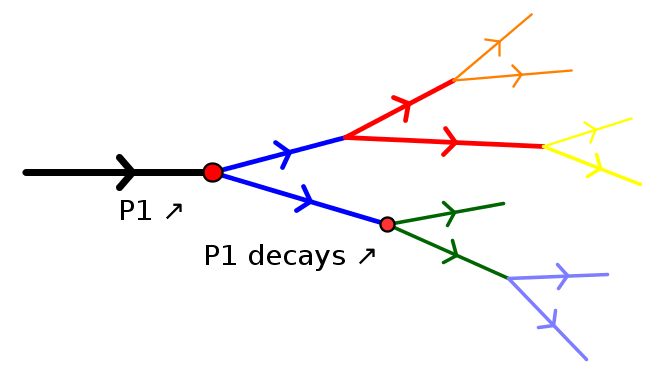
\includegraphics[scale=.3]{images/spilitting.png}
%\caption{Successive one-to-two splitting}\label{fig:partonshower}
%\end{figure} 
%\section{Hadronization}  

To reflect the colour neutrality of the particles in our model the partons will be transformed into a stable hadrons which are colour neutral. This process is called hadronization. The process in which this happens is not quantitatively well understood. For this model, a very simple approach is taken, where a direct translation between each parton and hadron is made. To achieve  this, a threshold energy is defined. Below it, the partons will begin to hadronize or stop splitting \citep{Salam:2010zt}. 
%The figure \ref{fig:hadronization} illustrate the process of splitting and hadronization.  
% The first implemented model and also follows Monte-Carlo event generators was Feynman-Field Model, which gives an idea of the formation of the mesons through iteratively from a single quark. However, this model is not collinear safe, which means the model can mix the short and long distance physics. Now a days two models are common, the string model and clustering model\citep{introduction}. 
%\begin{figure}
%\centering
%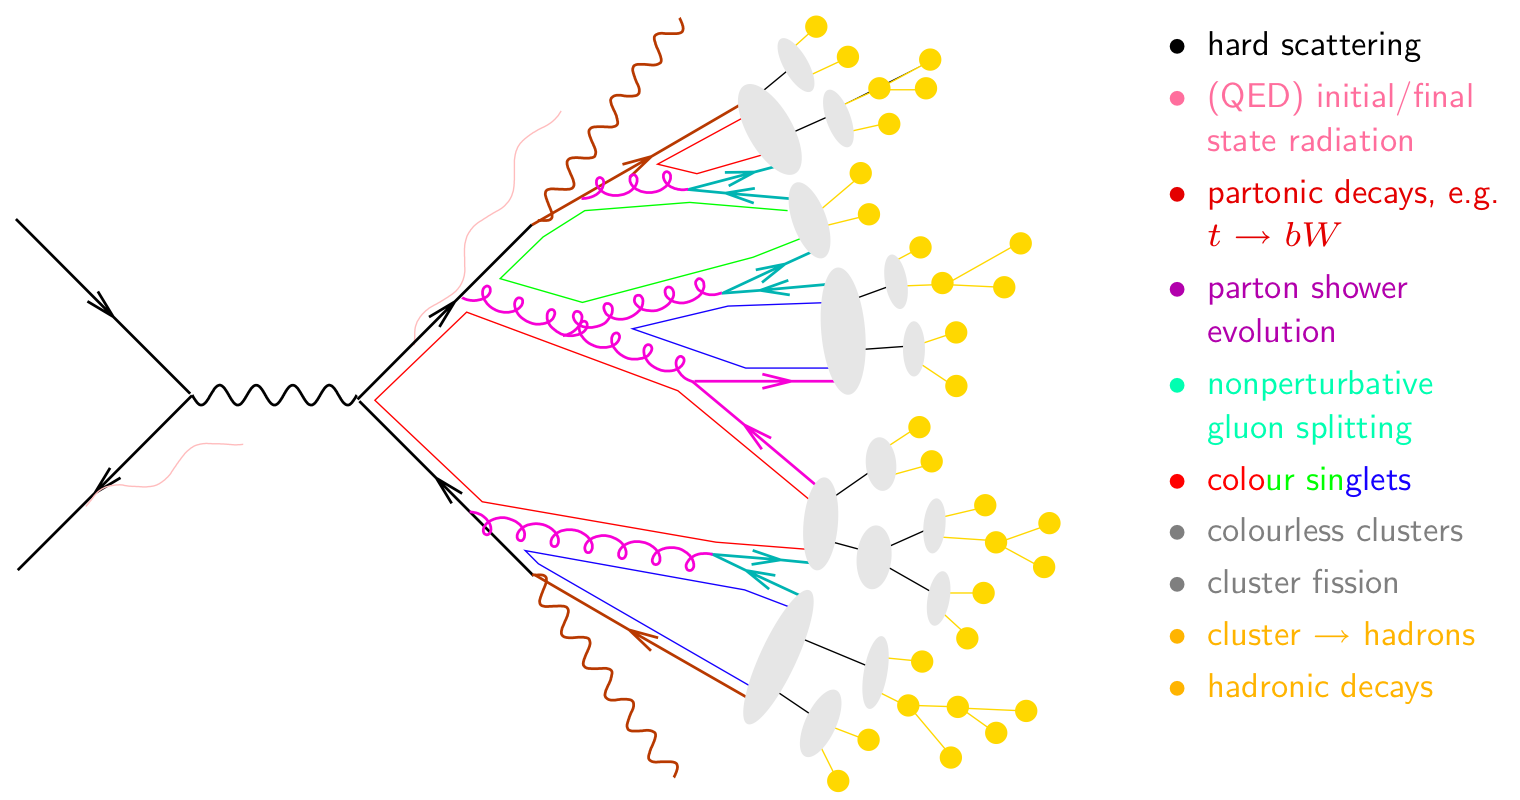
\includegraphics[scale=.4]{images/partonshower.png}
%\caption{Illustration of the subsequent dynamics of the parton shower (red and purple lines) and the hadronization (gray clusters and yellow circles) of the hard partons. Source (http://www.gk-eichtheorien.physik.uni-mainz.de/Dateien/Zeppenfeld-1.pdf) }\label{fig:hadronization}
%\end{figure}


\section{Parton Shower and Hadronization Simulation}

The following is a simple simulation for a splitting of a single particle into two. The parton shower simulation describes the parton shower and hadronization. The general idea of the two processes, parton shower and the hadonization can be simplified by the following algorithm
\begin{algorithmic}\label{logrithm}
\State Make list of particles $L$ 
\State Add initial particle $P_{i}$ to $L$
\State Define stability limit (hadronization limit) to be $S$  
\State While L is not empty
\If {energy of $P_{i} \geq  S$}
	\State Split into two and add to list and check again 
\Else 
	\State Begin hadronization  
\EndIf
\end{algorithmic}
This process can be simulated in two or three space dimensions, for the case of three dimensions, another quantity $\phi$ is needed.   

%\begin{figure}[]
%\centering
%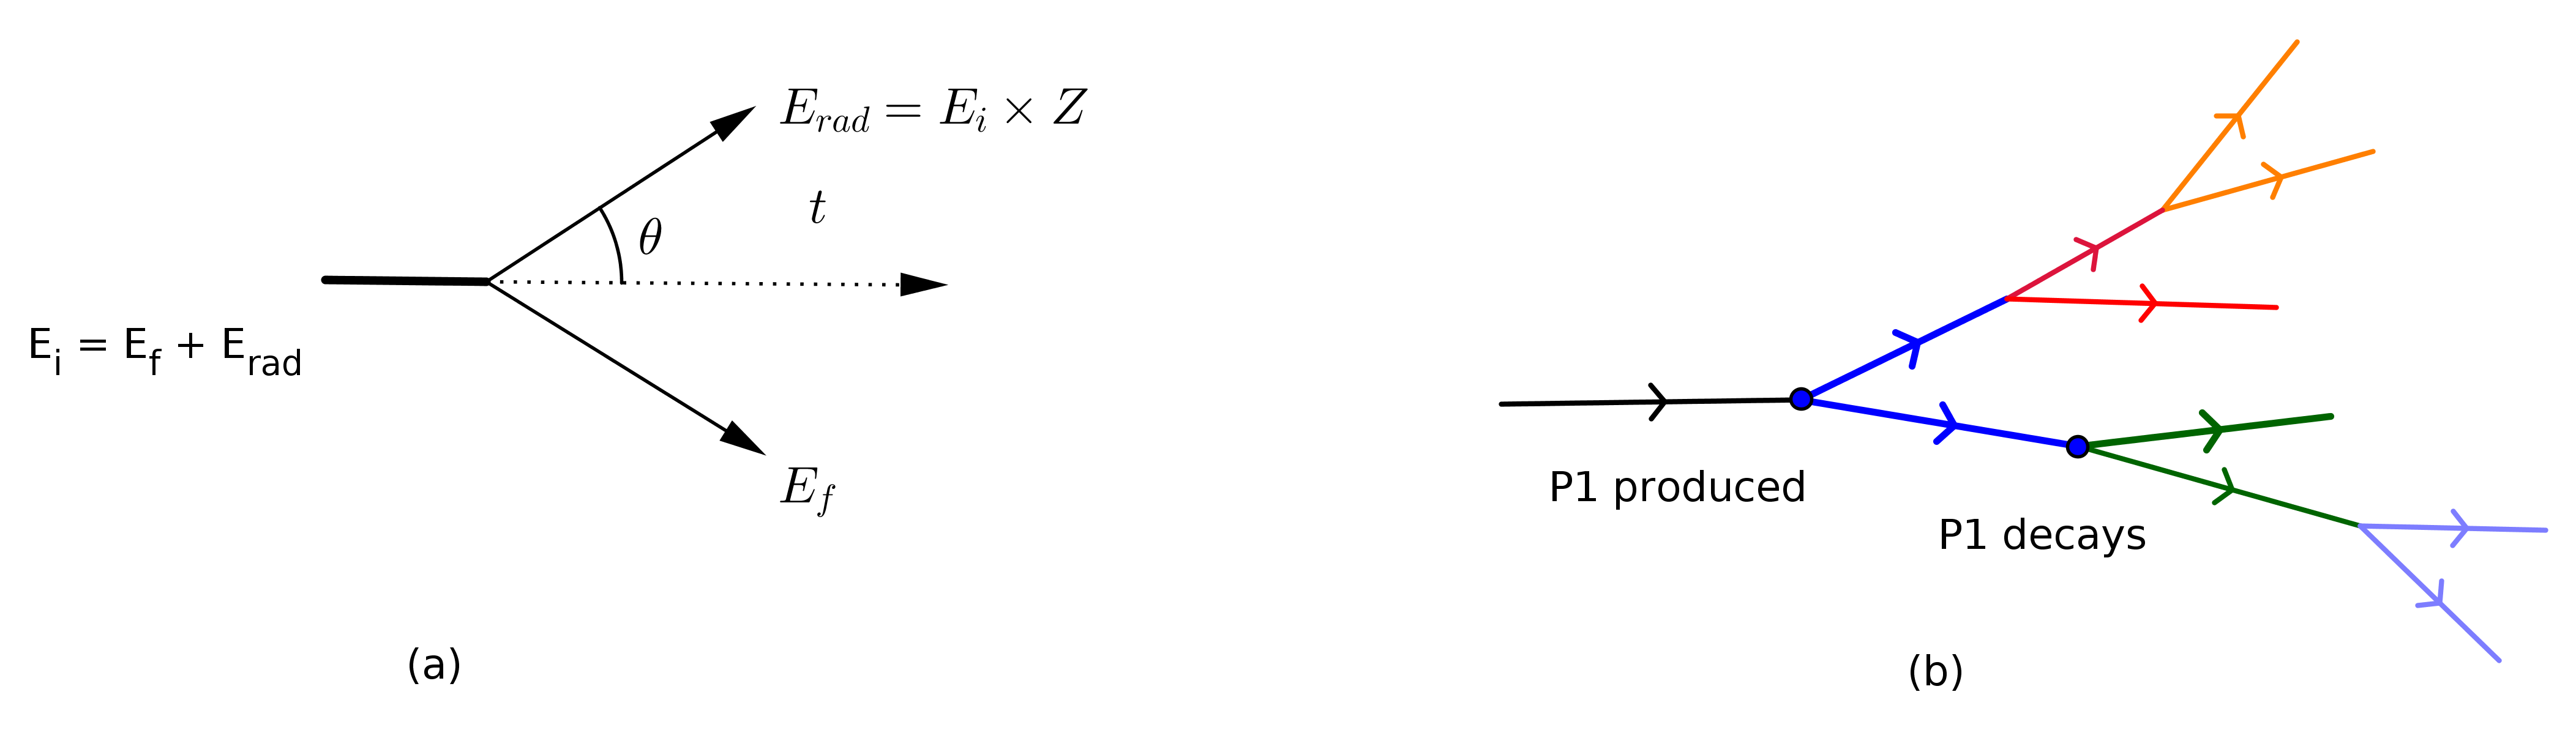
\includegraphics[scale=.12]{images/2d_spilitting.png}
%\caption{A single one-to-two splitting(a) highlighting one of the nodes in the composition of multiple splittings to form full parton shower(b).}
%\end{figure}
%
%\subsection{2-D Parton Shower}
%
%
%
%
%\Jnote{You need to make clear that in your model you do not make distinction
%  between quarks and gluons.}
%
%\Jnote{The picture with collision is way too small. Also caption is missing.}
%
%
%\subsection{3-D Parton Shower}
%
%
%\Jnote{OK, but you have to explain 3D case in detail. Consider making separate
%  sections for 2D and 3D. Picture showing what is angular (is this
%  correct name?) and azimuthal angle would be helpful.}
%
%\subsection{Implementation in python}
\section{Two Dimensions Parton Shower}
\begin{figure}[hbtp]
\centering
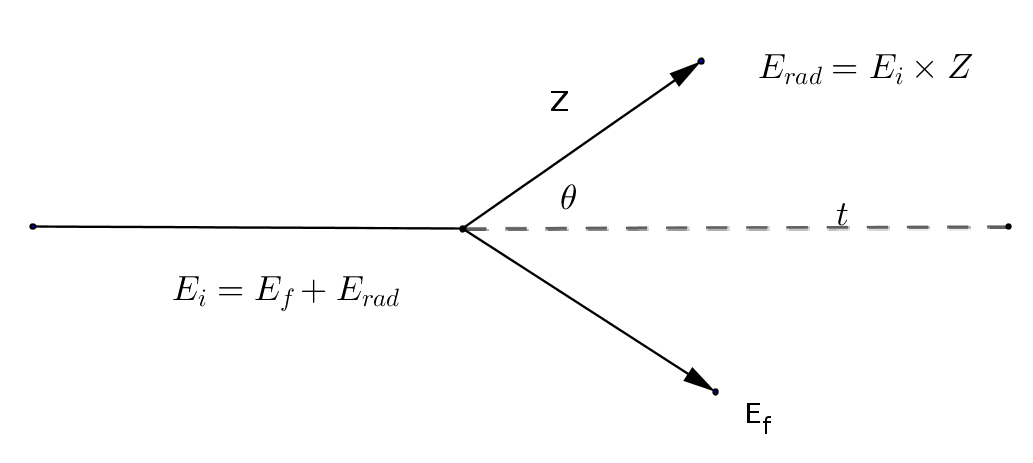
\includegraphics[scale=.35]{images/tt.png}
\caption{Illusration describing the splitting of a prticle into in two dimensions.}\label{fig:tt}
\end{figure}

The two dimensional model accounts for one rotation with angle $\theta$ (see figure \ref{fig:tt}). It evolves generation of two random numbers, one of them represent the angle and the other represents the energy of the radiated particle. Here, both the energy fraction $z$ and the angle $\theta$ are following the distribution $1/z$, this comes from the QCD approximation that was mentioned in \ref{sec}.  Where the former lies in the interval $[0, 1]$. To avoid the singularity at $z = 0$, a cutoff value of $\epsilon$ is added to the denominator by setting  $p(z) = \frac{1}{\epsilon + z}$. Considering the later in the interval [0,$\pi/2$], $\theta$ is modified in a similar way as $z$. The variables $\theta$ and $z$ are generated by applying the accept-reject method on a set of numbers that are uniformly distributed.

As for the kinematics description, the initial particle has four momentum $(E, p_{x}, p_{y},p_{z})$ \footnote{The four momentum vector is usually written as $(E/c, p_{x}, p_{y},p_{z})$. Henceforth, we are considering the natural units in which $c = 1$}, for simplicity we assume that the particle is travelling in $x$ direction with energy $E$. Therefore, the four momentum which describes this particle is the following 
\begin{equation}
P^{\mu}_{i}  = \begin{pmatrix}
E\\
p_x\\
0\\
0
\end{pmatrix}
\end{equation}
Where $p_y$ and $p_z$ are equal zero following our direction assumption. In a given splitting, with generated pair $(\theta, z)$, the kinematics of the radiated particle are determined.

To continue the showering process and to allow the model to proceed, it is necessary to determine the kinematics of the final state particle by applying the conservation of energy and momentum 
\begin{equation}
P_i^{\mu} = P_f^{\mu}
\end{equation}\label{conservation}

And Since \begin{equation}
P^{\mu} P_{\mu} = E^2 - (p_x^2 + p_y^2 + p_z^2) = E^2 - ||p|| = m_0^2
\end{equation} Which is lorentz invariant quantity, $i.e$, it does not depend on the frame. Here, we can make a simplifying assumption, in which we assume that the mass of the radiated particle is zero. This assumption is based on the fact that, in LHC the quark energy is $\sim$ 1$\si{MeV}$, where the hadron energy is $\sim$ 1 $\si{TeV}$. Now equation \ref{conservation} will become \begin{equation}\label{important}
E^2 = ||p||
\end{equation}\citep{Salam:2010zt}.    
  
In describing the direction of the radiated particle after it is being produced, we use the rotation matrix in two dimensions which rotates the radiated particle with the angle $\theta$ 
\begin{equation}
\begin{pmatrix}
\cos \theta & - \sin \theta\\
\sin \theta & \cos \theta
\end{pmatrix}
\end{equation}   

From this we can determine the direction of the other particle. Here we will denote its four momentum by $P_{part}^{\mu}$ . The final momentum  $P^{\mu}_{f}$ after the splitting is 
\begin{equation}
P_{rad}^{\mu} + P_{part}^{\mu}
\end{equation} and from the conservation equation \ref{conservation} then \begin{equation}
P^{\mu}_{i} = P_{rad}^{\mu} + P_{part}^{\mu}
\end{equation} Therefore, \begin{equation}
P_{part}^{\mu} = P^{\mu}_{i} - P_{rad}^{\mu} 
\end{equation}     

As in the algorithm \ref{logrithm}, a tunable parameter is made to account for the hadronization. The figure \ref{fig:2d} shows a graphical representation of the two dimensions parton shower as explained above. 
%For the python code see \verb+two_D_partonshower.py+.
     
%As for the four momentum vector, the module $numpy$ is used for this purpose, here we use the object $array$. \verb+Numpy+ is a scientific computing package in python which is widely used for these purposes, beside that it has powerful N-dimensional arrays it also has useful linear algebra tools and random number capabilities.         
%
%following the physical description a list contains the four momentum of the initial particle was defined, then we assumed that the particle has initial energy = 1 energy unit, since the particle will split after certain distance an assumption of the distance before the decay was made is that the particle will move a distance of 1 unit and then it will decay, basically it is an iteration process,  at the beginning we check the energy of the particle if it is a above the stability limit, which we assumed to $0.09$, this particle will split, the direction of the radiated will follow the $\theta$ and its energy will be given from $z$, and then both new particles four momenta will be add to the list at the beginning and again those particles will be checked, now if the particle has energy that is equal or below the stability limit then the iteration process will be terminated.   
%
%As for plotting the results, the library $matplotlib$ was used which is a library that is used to make 2 D plots in Python, as $matplotlib$ has the ability to add many lines at once, here the Linecollection is used, which is a package in $matplotlib$, the diagram in figure 3 shows the 2 D simulation of the parton shower.
\begin{figure}[hbtp]
\centering
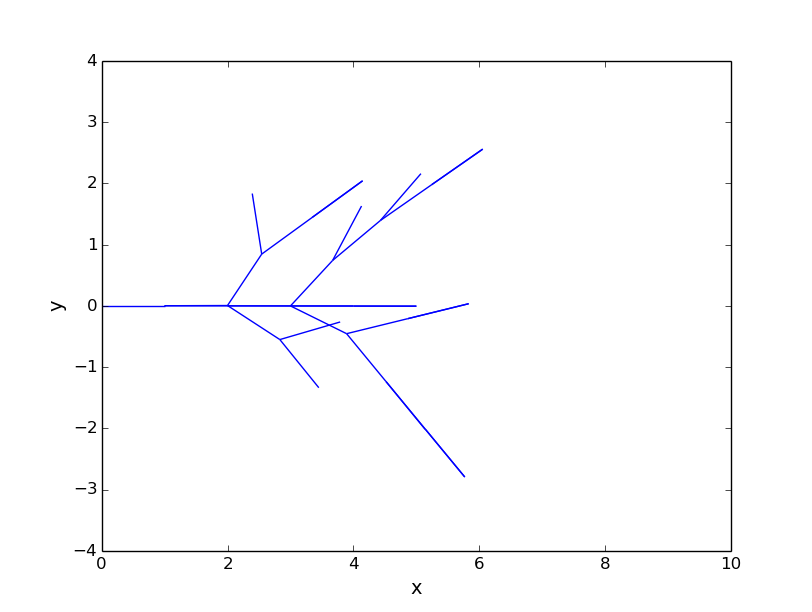
\includegraphics[scale=.6]{images/2D_partonshower.png}
\caption{A two dimesions simulation of the spliting of a single parton.}\label{fig:2d}
\end{figure}

\section{Three Dimensions Parton Shower}

\begin{figure}[hbtp]
\centering
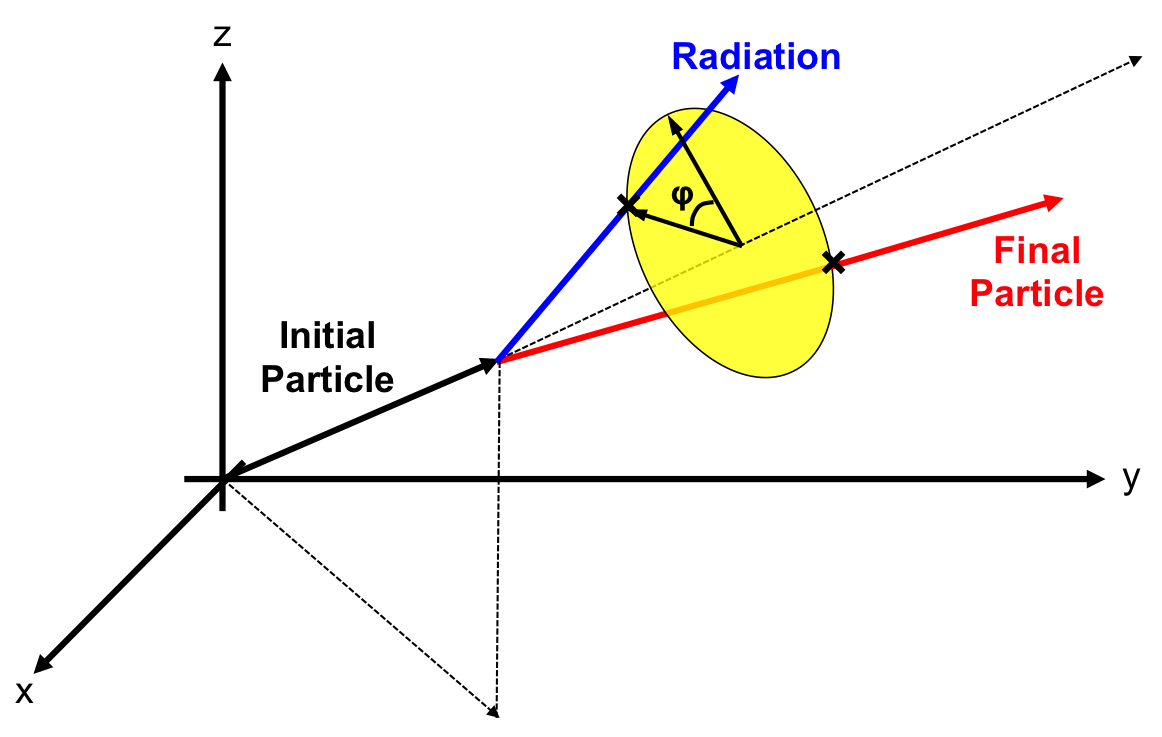
\includegraphics[scale=.5]{images/three-dimentions.png}
\caption{An illustration of the azimuthal angle $\phi$ of a one-to-two splitting occurring in three dimensions.}\label{fig:3d}
\end{figure}
Since the real physics we are modelling is in three dimension, we need to modify our model to account for this. An additional splitting angle $\phi$ will be included, which is the azimuthal angle of the decay  around the direction of travel of the initial particle, as shown in figure \ref{fig:3d}.

Unlike the angle $\theta$, there is no preference for the value of this angle and it should therefore be chosen from a uniform distribution within the interval $[0,2\pi]$ \citep{Salam:2010zt}.

There are no major differences between the three and two dimensional models, except that in the three dimensional model the particle will be rotated twice with the angles $\theta$ and $\phi$. Given a unit vector \textbf{u}, where \textbf{u} is the vector in the direction of the axis of rotation,  the rotation around the axis by angle $\theta$ can by found by matrix       
\begin{equation} 
\begin{pmatrix}
\cos\theta + u^2_x(1-\cos\theta) & u_x u_y (1-\cos\theta) - u_z \sin\theta& u_x u_z(1-\cos\theta)+ u_y \sin\theta\\

u_y u_x (1 - \cos\theta) + u_z \sin\theta & \cos\theta + u_y^2 (1 - \cos\theta) & u_y u_z (1 - \cos\theta) - u_x \sin\theta \\

u_z u_x (1 - \cos\theta) - u_y \sin\theta & u_z u_y (1 - cos\theta) + u_x \sin\theta & \cos\theta + u_z^2 (1 - \cos\theta)
\end{pmatrix}
\end{equation}

First the momentum vector is rotated angle $\theta$ around an arbitrary axis that is perpendicular to it, after that the resulting vector is rotated around the original vector with the angle $\phi$.  
The figure \ref{fig:3dparton} shows a graphical representation of the three dimensional parton shower. 
%For the python code see \verb+partonshower3d.py+.

%The 3D simulation of the parton shower is essentially the same as for python code with few changes, in which now we have two rotation angles, $\theta$ and also $\phi$ which is the azimuthal angle which is uniformly distributed in the interval [0,2$\pi$]. To simulate the rotation in three dimensions, the function \verb+normv(u)+ and function \verb!rotation(v,angle)!, the former returns the axis of the rotation, the function input and the vector [1,1,1] from a plane, from which we find a vector that is orthogonal to this plane, and the later is matrix of rotation, it takes the angle rotation and the axis of rotation as inputs. 
%
%Also here z (the energy fraction) now is lies the interval[0,1] and the stability limit is 0.05. The digram in figure 4 shows the 3D simulation of single parton splitting.
%
%\Jnote{This description (both 2D and 3D case) should be way longer,
%  more organized and more detailed. It should take several pages and you
%  should explain what the code is doing precisely and in detail.}
% 
\begin{figure}[H]
\centering
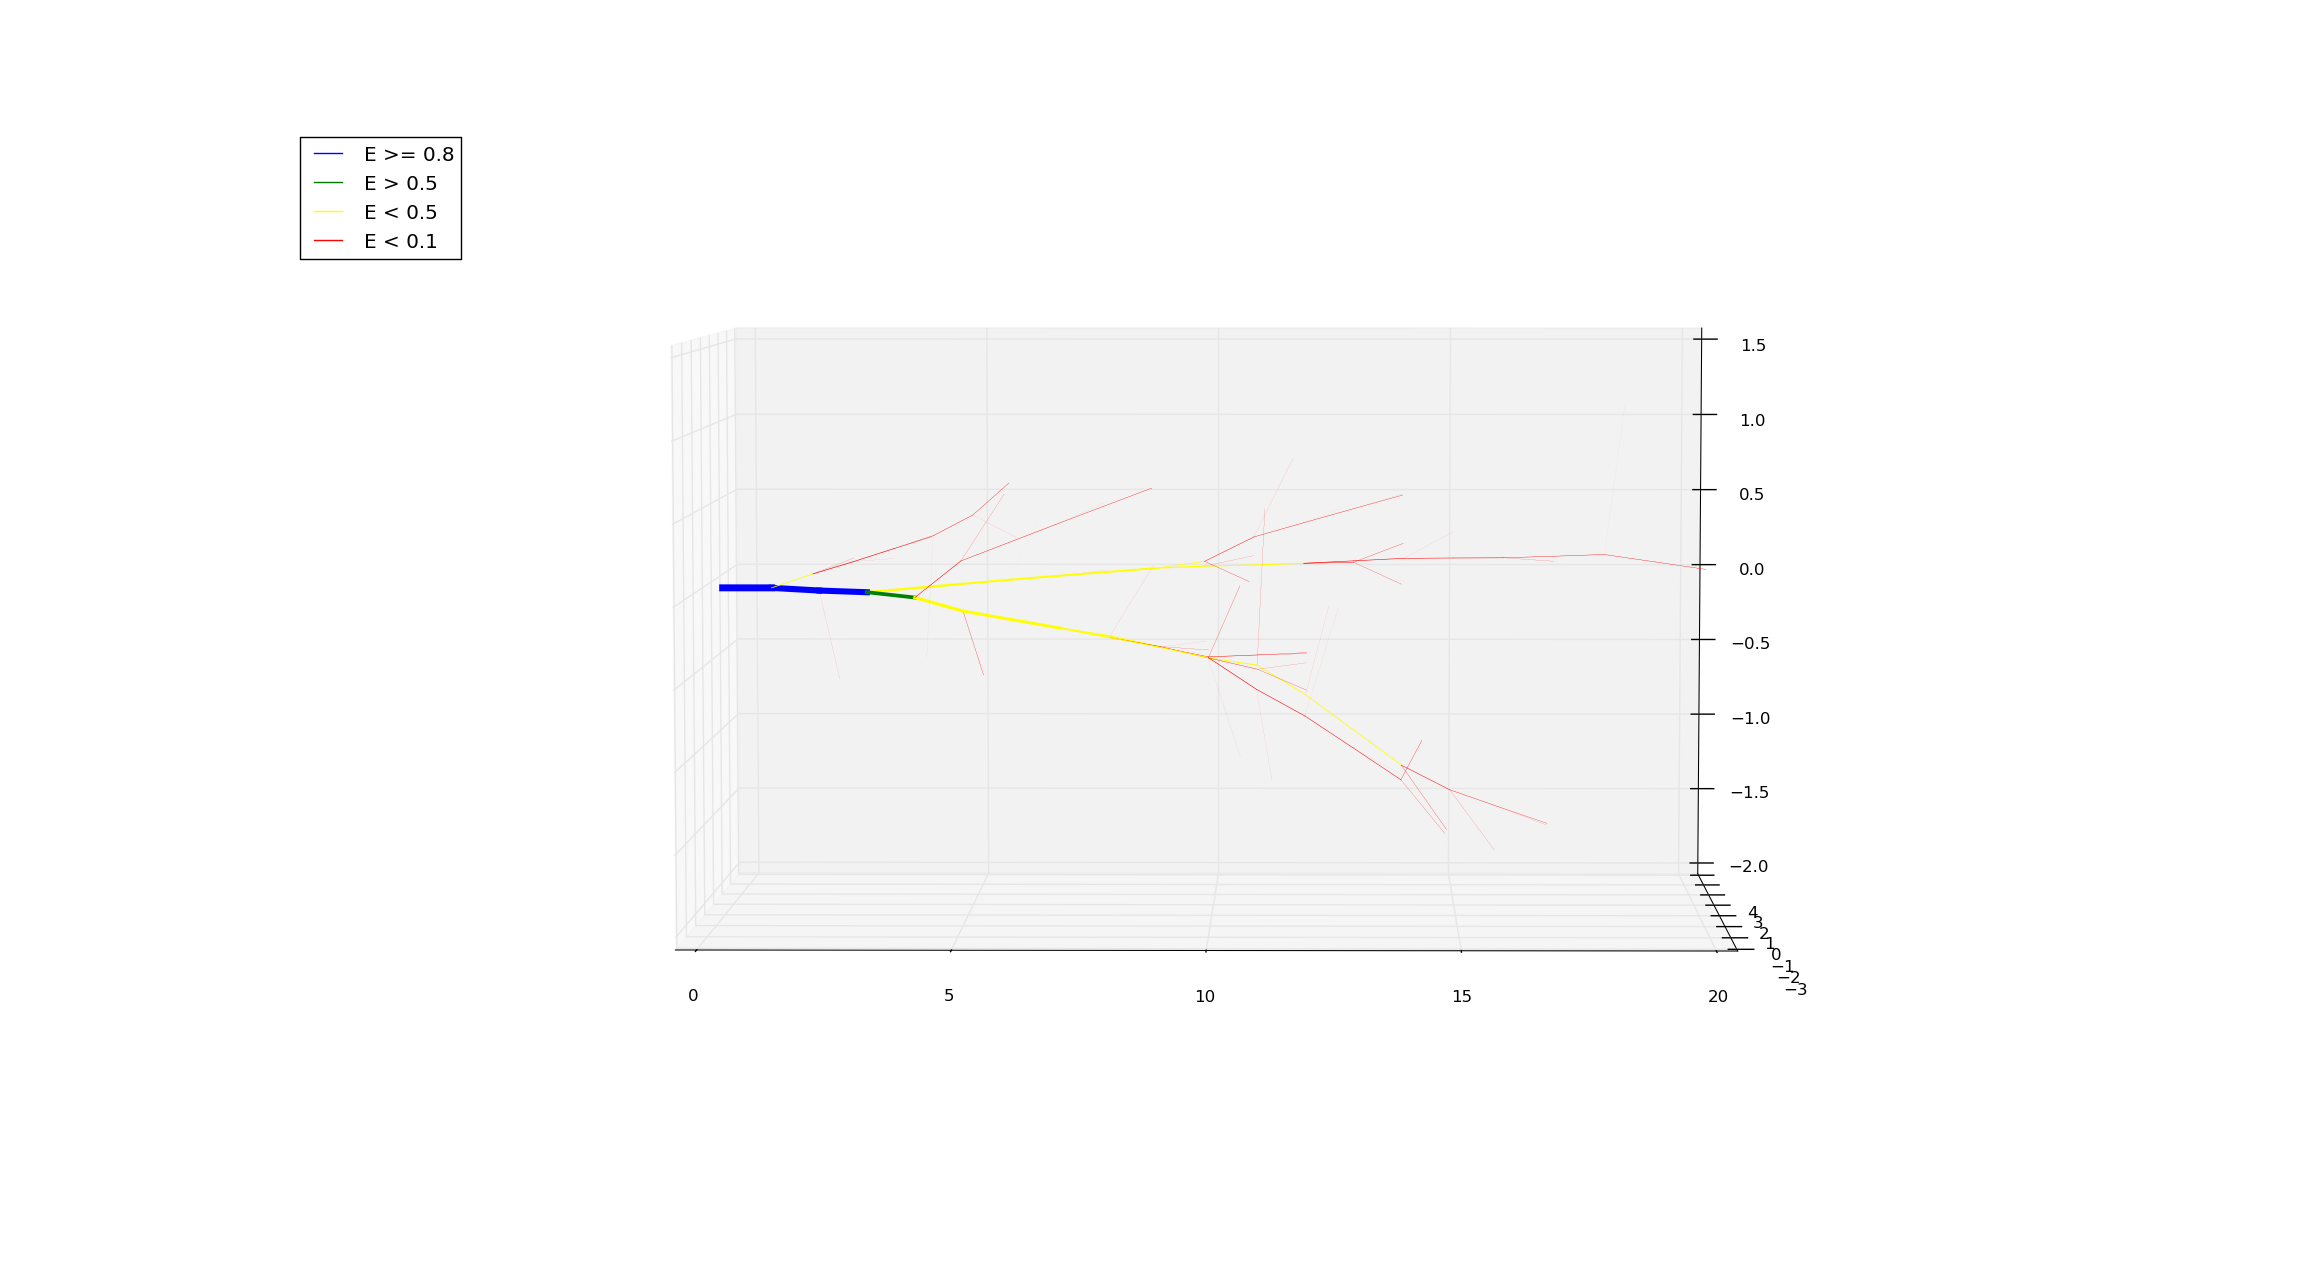
\includegraphics[scale=.3]{images/3D_partonshower.png}
\caption{A three dimensions simulation of the spliting of a single parton. In this ilustraion the blue colour represents the paricles with energy $\geq 0.8$, the green colour represnts the particles with energy $\geq 0.5$, the yellow colour represents the particles with energy $\leq 0.5$ and the red colour represents the particles with energy $\leq 0.1$.}\label{fig:3dparton}
\end{figure}
%
%\begin{figure}[hbtp]
%\centering
%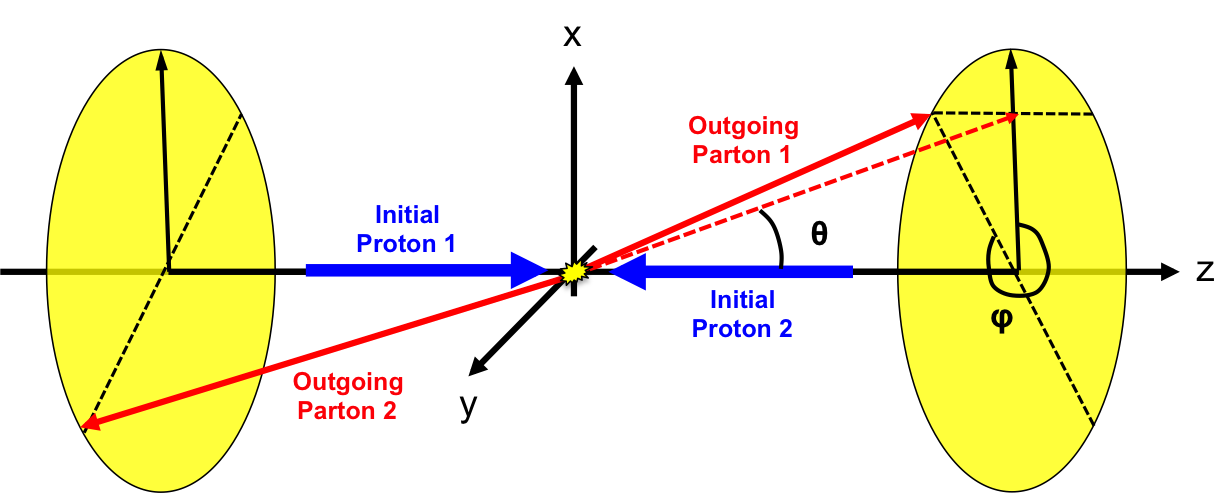
\includegraphics[scale=.3]{images/twoparticles.png}
%\caption{Illustration representation of a proton-proton collision event similar to that in the LHC.}\label{fig:twopartons}
%\end{figure}
\section{An Improved Model}
In order to build more realistic model, it is necessary to include more details, as we did with the three dimensions model. Here we start by looking at the particle in the moment of production, right after the collision of the two protons. For simplicity One can assume that the collision of the protons conserves the momentum. Hence the produced particle also conserve momentum. Following this assumption, it can be said the produced particles come in pairs that have opposite directions. The produced particles have energy that is randomly distributed as well as the polar angle $\theta$ and the azimuthal $\phi$ angle. As for the energy, it has the exponential distribution $e^{- \alpha E_{parton}}$, where $\alpha$ is a physically meaningful parameter that characterizes the collisions at the LHC and $E_{parton}$ is randomly chosen energy of the parton. As for the polar and the azimuthal angles, the collision has no preferred angle in terms of the both angles $\theta$ and $\phi$ as shown in figure \ref{fig:twopartons}, hence, the former is uniformly distributed in the range $[0, \pi]$ and the later is uniformly distributed in the range $[0,2 \pi]$. \citep{Salam:2010zt}.  
%In the LHC collision, usually two partons are emitted, it is very rare to produce a single parton. Since the collision was between two particles travelling opposite to each other, a simplification assumption can be made. That the particles are in a configuration that conserve the momentum, this is as a result of the initial momentum $= 0$. There are some aspects of this configuration which are stochastic, these are :
%\begin{itemize}
%\item[•]
%Energy : the emitted particle has a randomly distributed  energy which falls under the exponential distribution $e^{- \alpha E_{parton}}$, where $\alpha$ is a physically meaningful parameter that characterizes the collisions at the LHC and $E_{parton}$ is randomly chosen energy of the parton. 
%\item[•]
%The azimuthal and the polar direction. The collision has no preferred angle in terms of the both angles $\theta$ and $\phi$ as shown in figure \ref{fig:twopartons}, hence, the former is uniformly distributed in the range $[0, \pi]$ and the later is uniformly distributed in the range $[0,2 \pi]$ \citep{Salam:2010zt}.    
%\end{itemize}
%


There are three main programs in use at present for the generation of simulated collider events. They incorporate different combinations of the approaches of the model described above. These are HERWIG, PYTHIA and SHERPA \citep{Buckley:2011ms}.      